\begin{tikzpicture}
\tikzset{
    overlay box/.style={fill=white,fill opacity=0.9}
}
\node[overlay,anchor=north west,inner sep=0mm] (base) at (0, 0) {
    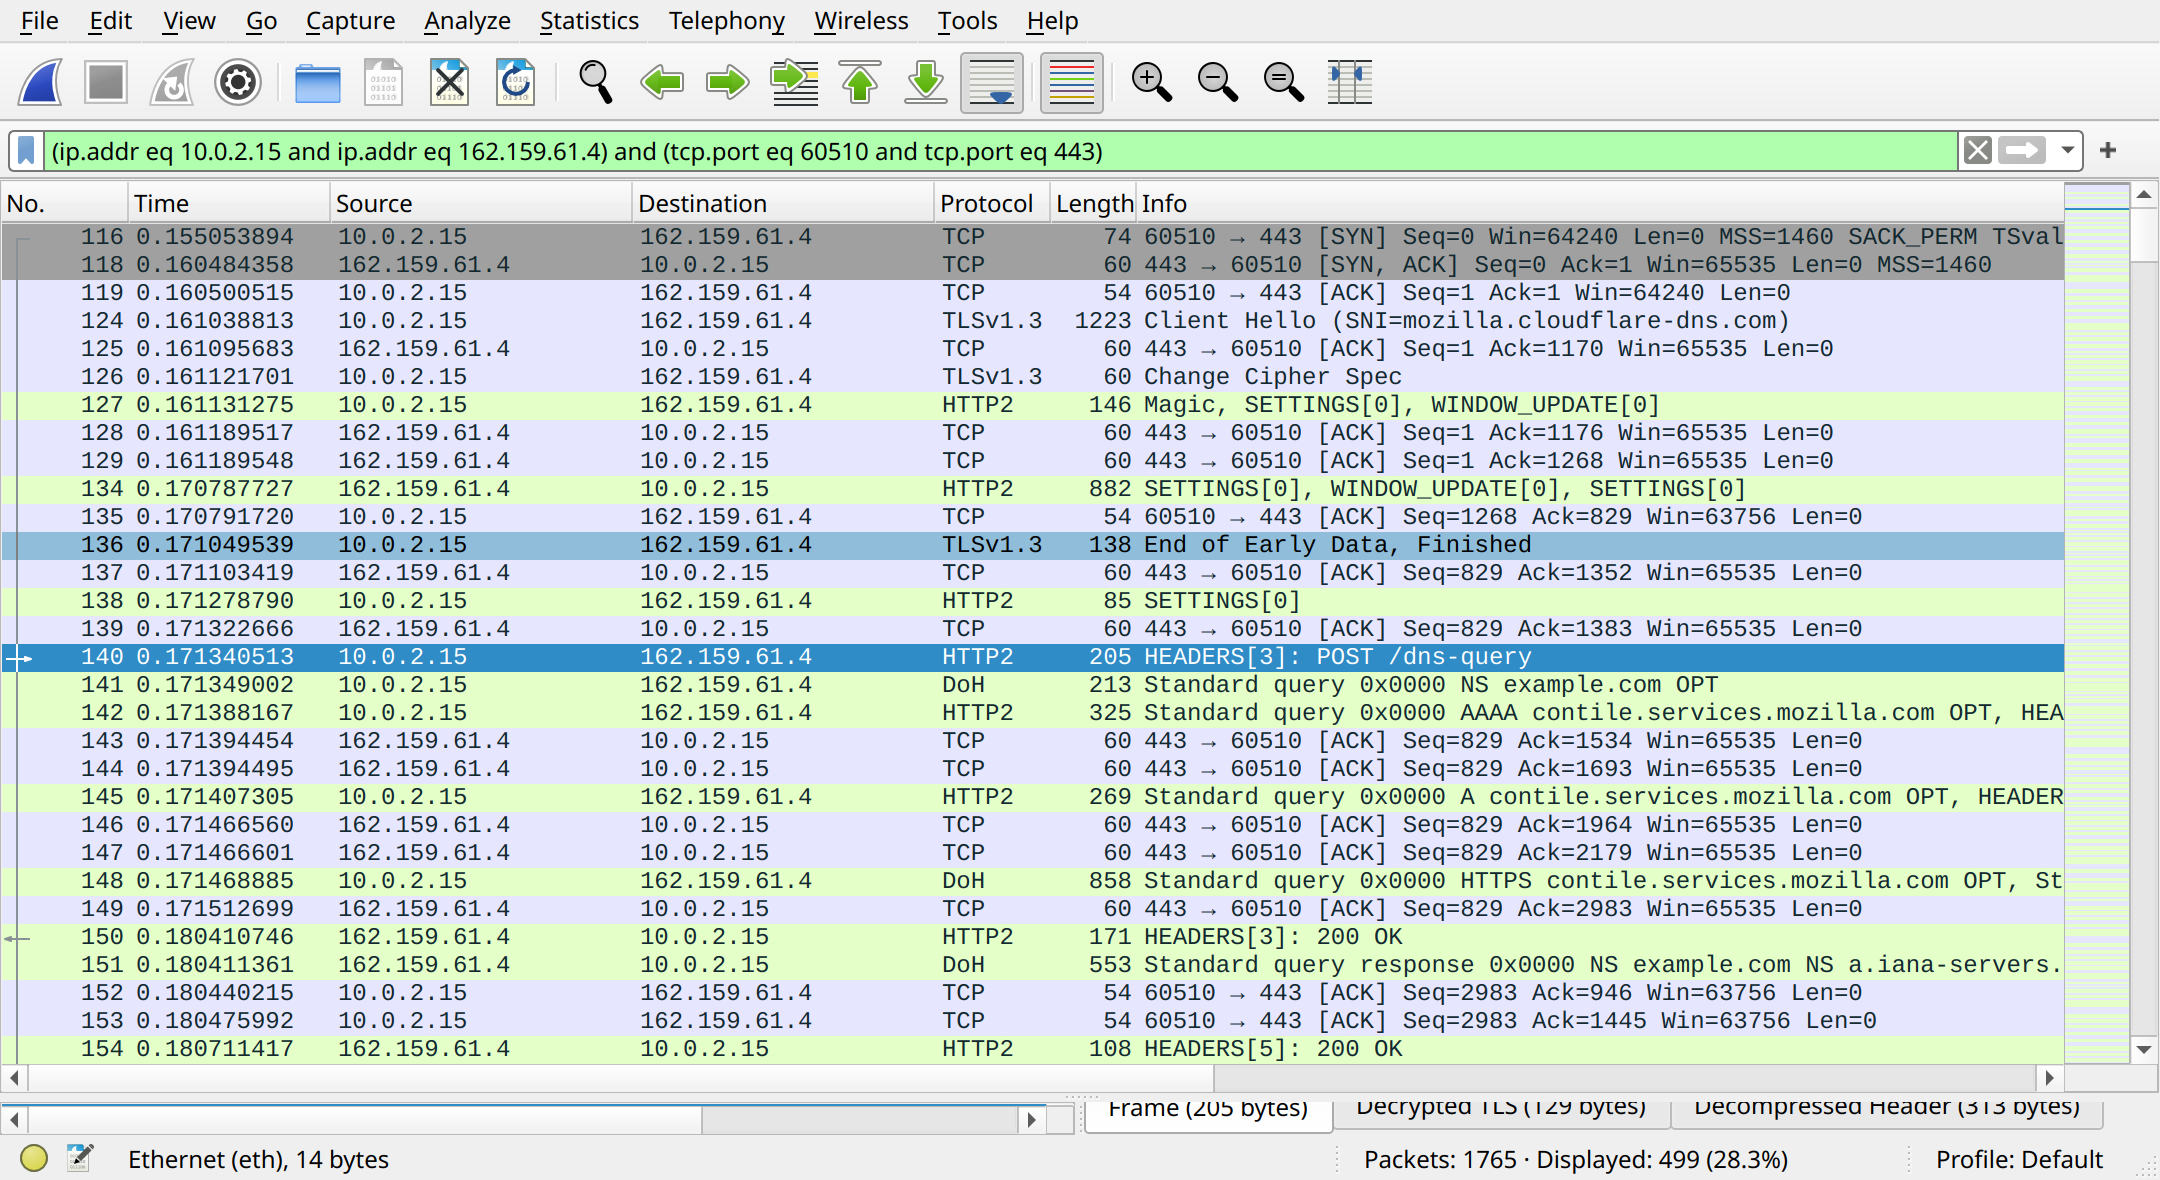
\includegraphics[width=\mypaperwidth]{../intro/wireshark-filtered.png}
};
\path (0, 0) rectangle (14.5, -7); % for bounding box
%\draw[overlay,help lines] (0, 0) grid (14, -8);
%\draw[overlay,help lines,dotted] (0, 0) grid[step=0.2] (14, -8);
\begin{visibleenv}<1>
    \path[draw, red, very thick] (0.3, -0.9) rectangle (13.15, -1.15);
    \node[anchor=north,overlay box,text=red] (filter expr label) at (6.5, -1.15) {
        filter expression 
    };
    \node[anchor=north,overlay box,font=\fontsize{10}{11}\selectfont,align=left] at (filter expr label.south) {
        based on address ($\sim$ machine) and port number ($\sim$ program/socket) fields  \\
        usually means all part of one socket connection
    };
    \path[draw, red, very thick] (10.3, -7.6) rectangle (12.1, -7.9);
    \node[anchor=south,overlay box,text=red] at (11.4, -7.6) {
        499 packets in ``conversation''
    };
\end{visibleenv}
\begin{visibleenv}<2>
    \path[draw,red, very thick] (0, -1.9) rectangle (.85, -2.24);
    \path[draw,red, very thick] (0, -3) rectangle (.85, -3.37);
    \node[overlay box,anchor=west,text=red] at (.85, -2.5) {
        some packets not shown from filter
    };
\end{visibleenv}
\begin{visibleenv}<3>
    \path[draw,red,very thick] (6.25, -1.47) rectangle (7.1, -7.2);
    \node[align=left,overlay box,anchor=south east,text=red] at (6.25, -3) {
        highest layer used \\
        in each packet
    };
    \node[align=left,overlay box,anchor=north east,text=black,font=\fontsize{10}{11}] at (6.25, -3) {
        connection only `for' \\
        DNS over HTTPS (DoH) \\
        but many packets \\
        only needed for \\
        bookkeeping for \\
        the `lower' layers
    };
\end{visibleenv}
\begin{visibleenv}<4>
    \path[draw,red,very thick] (2.2, -1.47) rectangle (6.25, -7.2);
    \node[align=left,overlay box,anchor=west] at (6.25, -4) {
        bookkeeping packets sent \\
        in both directions
    };
\end{visibleenv}
\end{tikzpicture}